\documentclass[11pt]{article}
\usepackage{geometry}                % See geometry.pdf to learn the layout options. There are lots.
\geometry{a4paper}                   % ... or a4paper or a5paper or ... 
%\geometry{landscape}                % Activate for for rotated page geometry
%\usepackage[parfill]{parskip}    % Activate to begin paragraphs with an empty line rather than an indent
\usepackage{graphicx}
\usepackage{amssymb}
\usepackage{amsmath}
\usepackage{lipsum}
\usepackage{authblk}
%\usepackage{amsaddr}
\usepackage{epstopdf}
\usepackage{booktabs}
\usepackage{bbold}
\usepackage{bm}
\usepackage{xcolor}
\usepackage{fancyhdr}
\usepackage[yyyymmdd,hhmmss]{datetime}
\pagestyle{fancy}
\rfoot{Compiled on \today\ at \currenttime}
\cfoot{}
\lfoot{Page \thepage}
\RequirePackage[colorinlistoftodos,prependcaption,textsize=tiny]{todonotes} % look for '\todo'
\definecolor{darkred}{rgb}{0.4,0.0,0.0}
\definecolor{darkgreen}{rgb}{0.0,0.4,0.0}
\definecolor{darkblue}{rgb}{0.0,0.0,0.4}
\usepackage[bookmarks,linktocpage,colorlinks,
    linkcolor = darkred,
    urlcolor  = darkblue,
    citecolor = darkgreen]{hyperref}

%\DeclareGraphicsRule{.tif}{png}{.png}{`convert #1 `dirname #1`/`basename #1 .tif`.png}

\renewcommand{\headrulewidth}{0pt}
\fancyhead[L]{
%\includegraphics[width=4cm]{/Users/tomluu/Research/talks/fzjTemplate/uniBonn_logo.jpg}
}
\fancyhead[R]{

\includegraphics[width=4cm]{figs/fzj_logo.jpg}
}
\pagestyle{plain}

\title{Understanding finite-volume corrections to spherical L\"uscher}
\author[1,2]{Thomas Luu}
\affil[1]{Institute for Advanced Simulation 4\\
Forschungszentrum J\"ulich, Germany}
\affil[2]{Rheinische Friedrich-Williams-Universit\"at Bonn, Germany}

%\email{t.luu@fz-juelich.de}
\date{}                                           % Activate to display a given date or no date


\begin{document}
\maketitle
\begin{center}
email: \href{mailto:t.luu@fz-juelich.de}{t.luu@fz-juelich.de}
\end{center}
\abstract{
Ok, I show that the L\"uscher dispersion formula is equivalent to solving the Schr\"odinger equation, and derive the linear and quadratic behavior found when using the spherical L\"uscher formula with contact interaction.
}

\thispagestyle{fancy}

\clearpage{}
%\tableofcontents
%\newpage

\section{Dispersion L\"uscher (with contact interaction) is really the Schr\"odinger equation in disguise\label{sect:disguise}}

Ok, I assume I live in a cubic box of side length $L$ and space is discretized with lattice spacing $\epsilon$ corresponding to $N$ sites per side. Also, I only have a contact interaction for the time being,
\begin{equation}
\langle \bm n|\hat V|\bm m\rangle = C_0(\Lambda)\ .%\Theta\left(|\bm n|-\frac{\Lambda L}{2\pi}\right)\Theta\left(|\bm m|-\frac{\Lambda L}{2\pi}\right)\ .
\end{equation}
For now I don't assume anything about $\Lambda$, i.e. I treat it as just some parameter.  The states $|\bm n\rangle$ are eigenvectors of the non-interacting Hamiltonian\footnote{I assume an $n_{step}=\infty$ dispersion, but the results of this section also hold for finite $n_{step}$.},
\begin{equation}
\hat H_0|\bm n\rangle = \frac{4\pi^2}{mL^2}\bm n^2|\bm n\rangle\ .
\end{equation}
The Schr\"odinger equation with this interaction is
\begin{equation}\label{eqn:schroedinger}
\left(\hat H_0+\hat V\right)|\psi\rangle = E|\psi\rangle\ ,
\end{equation}
where $|\psi\rangle$ is an eigenstate and $E$ is its corresponding eigenvalue.  I now put eq.~\eqref{eqn:schroedinger} into its integral form,
\begin{equation}\label{eqn:integral form 1}
|\psi\rangle = \frac{1}{E-\hat H_0}\hat V|\psi\rangle\ ,
\end{equation}
and act with $\langle \bm n|$ from the left,
\begin{equation}\label{eqn:integral form 2}
\langle \bm n|\psi\rangle = \frac{1}{E-\frac{4\pi^2}{mL^2}\bm n^2}\langle \bm n|\hat V|\psi\rangle\ .
\end{equation}
Note that the closure relation in a discretized box is
\begin{equation}\label{eqn:closure}
\hat 1=\frac{1}{L^3}\sum_{\bm n \in (-N/2,N/2]^3}|\bm n\rangle \langle \bm n|=\frac{1}{L^3}\sum_{\bm n \in \mathrm{B.Z.}}|\bm n\rangle \langle \bm n|\ .
\end{equation}
I simplify notation by replacing $\bm n \in (-N/2,N/2]^3$ with $\bm n \in\mathrm{B.Z.}$ where B.Z. stands for 1st Brillouin Zone. So now I insert a complete set of states into eq.~\eqref{eqn:integral form 2},
\begin{multline}\label{eqn:integral form 3}
\langle \bm n|\psi\rangle =\frac{1}{L^3} \sum_{\bm m\in\mathrm{B.Z.}}\frac{1}{E-\frac{4\pi^2}{mL^2}\bm n^2}\langle \bm n|\hat V|\bm m\rangle \langle \bm m|\psi\rangle\\
=\frac{1}{L^3} \sum_{\bm m\in\mathrm{B.Z.}}\frac{C_0(\Lambda)}{E-\frac{4\pi^2}{mL^2}\bm n^2} \langle \bm m|\psi\rangle\ .
\end{multline}
I now sum over all vectors $\bm n$ in the first B.Z.,
\begin{multline}
\sum_{\bm n\in \mathrm{B.Z.}}\langle \bm n|\psi\rangle =\frac{1}{L^3} \sum_{\bm n,\bm m\in\mathrm{B.Z.}}\frac{C_0(\Lambda)}{E-\frac{4\pi^2}{mL^2}\bm n^2} \langle \bm m|\psi\rangle\\
=\sum_{\bm m\in \mathrm{B.Z.}}\langle \bm m|\psi\rangle\frac{1}{L^3} \sum_{\bm n\in\mathrm{B.Z.}}\frac{C_0(\Lambda)}{E-\frac{4\pi^2}{mL^2}\bm n^2}\ .
\end{multline}
I can now move everything to the LHS (and rename some dummy variables),
\begin{equation}
\sum_{\bm m\in \mathrm{B.Z.}}\langle \bm m|\psi\rangle\left(1-\frac{1}{L^3} \sum_{\bm n\in\mathrm{B.Z.}}\frac{C_0(\Lambda)}{E-\frac{4\pi^2}{mL^2}\bm n^2}\right)=0\ .
\end{equation}
So this expression holds if\footnote{The expression also holds if
\begin{displaymath}
\sum_{\bm m\in \mathrm{B.Z.}}\langle \bm m|\psi\rangle=0\ ,
\end{displaymath}
but I believe that such a condition cannot be true in general.  Can someone prove this?}
\begin{align}
1-&\frac{1}{L^3} \sum_{\bm n\in\mathrm{B.Z.}}\frac{C_0(\Lambda)}{E-\frac{4\pi^2}{mL^2}\bm n^2}=0\nonumber\\
\implies& \frac{-1}{C_0(\Lambda)}=\frac{1}{L^3}\sum_{\bm n\in\mathrm{B.Z.}}\frac{1}{\frac{4\pi^2}{mL^2}\bm n^2-E}\ .\label{eqn:almost there}
\end{align}
I manipulate eq.~\eqref{eqn:almost there} just a little to make it look more familiar,
\begin{equation}
 \frac{-4\pi/m}{C_0(\Lambda)}=\frac{1}{\pi L}\sum_{\bm n\in\mathrm{B.Z.}}\frac{1}{\bm n^2-x}\ .\label{eqn:really almost there}
 \end{equation}
 where 
 \begin{equation}
 x\equiv \frac{mEL^2}{4\pi^2}\ .
 \end{equation}
\emph{Given some coefficient $C_0(\Lambda)$ for the delta interaction, the (dimensionless) eigenvalues $x$ that satisfy Schr\"odinger's equation~\eqref{eqn:schroedinger} (with this interaction) will also satisfy the self-consistent equation~\eqref{eqn:really almost there}.  This is because eq.~\eqref{eqn:really almost there} and eq.~\eqref{eqn:schroedinger} are really the same thing.  This holds for \emph{any} $C_0(\Lambda)$.}

Of course we tune $C_0(\Lambda)$ to reproduce some observable in the infinite-volume limit, which in this case is the scattering length $a_0$,
\begin{equation}\label{eqn:C0(lambda)}
C_0(\Lambda)=\frac{-4\pi/m}{\frac{-1}{a_0}+\mathcal{L}^\square_3\frac{\Lambda}{4\pi^2}}\ ,
\end{equation}
where $\mathcal{L}^\square_3=15.348248444887464047104634$. I now identify the cutoff $\Lambda$ with the lattice spacing $\epsilon$,
\begin{equation}
\frac{1}{\epsilon}=\frac{\Lambda}{2\pi}=\frac{N}{L}\ ,
\end{equation}
allowing me to trade $\Lambda$ for the ratio $N/L$ in eq.~\eqref{eqn:C0(lambda)},
\begin{equation}\label{eqn:C0(N)}
C_0(N/L)=\frac{-4\pi/m}{\frac{-1}{a_0}+\mathcal{L}^\square_3\frac{N}{2\pi L}}\ .
\end{equation}
Plugging this expression into eq.~\eqref{eqn:really almost there} gives the desired result,
\begin{equation}\label{eqn:finally there}
\frac{-1}{a_0}=\frac{1}{\pi L}\left(\sum_{\bm n\in\mathrm{B.Z.}}\frac{1}{\bm n^2-x}-\mathcal{L}^\square_3\frac{N}{2}\right)\quad\quad\left(=\frac{1}{\pi L}S^{\square N}_3(x)\right)\ .
\end{equation}
I stress again:  for the coefficient of the delta function interaction given by eq.~\eqref{eqn:C0(N)}, the eigenvalues $x$ of the Schr\"odinger equation with this interaction will exactly satisfy the relation in eq.~\eqref{eqn:finally there}, which is our dispersion L\"uscher formula.  

\section{Corrections to the spherical L\"uscher formula (with contact interaction)}
What happens when one takes values of $x$, calculated with a delta function interaction in a box of side length $L$ with $N$ points per side, and plugs it instead into the spherical L\"uscher formula\footnote{Here I must constrain myself to an $n_{step}=\infty$ analysis.  Maybe there's a way to do this with finite $n_{step}$?},
\begin{equation}\label{eqn:spherical luscher}
\frac{1}{\pi L}S^\bigcirc_3(x)=\lim_{\eta \to\infty}\frac{1}{\pi L}\left(\sum_{\bm n}^{|\bm n|<\eta / 2} \frac{1}{\bm n^{2}-x}-\mathcal{L}^\bigcirc_3\frac{\eta}{2}\right)\ \ ?
\end{equation}
Here $\mathcal{L}^{\bigcirc}_3\equiv 4\pi$.  Let's find out\ldots

I can separate out the dispersion L\"uscher formula from eq.~\eqref{eqn:spherical luscher} by adding and subtracting it,
\begin{multline}
\frac{1}{\pi L}S^\bigcirc_3(x)=\frac{1}{\pi L}\left(S^{\square N}_3+\left(S^\bigcirc_3(x)-S^{\square N}_3\right)\right)=\frac{-1}{a_0}+\frac{1}{\pi L}\left(S^\bigcirc_3(x)-S^{\square N}_3\right)\\
=\frac{-1}{a_0}+\lim_{\eta \to\infty}\frac{1}{\pi L}\left(\sum_{\bm n\notin \mathrm{B.Z.}}^{|\bm n|<\eta / 2} \frac{1}{\bm n^{2}-x}-\mathcal{L}^\bigcirc_3\frac{\eta}{2}+\mathcal{L}^\square_3\frac{N}{2}\right)
\end{multline}
Since $\bm n$ is now restricted to be \emph{outside} the B.Z., I can assume that $\bm n^2\gg x$ which allows me to Taylor expand under the summation,
\begin{align}
S^\bigcirc_3(x)=&\frac{-\pi L}{a_0}\label{eqn:observable}\\
&+\mathcal{L}^\square_3\frac{N}{2}+\lim_{\eta \to\infty}\left(\sum_{\bm n\notin \mathrm{B.Z.}}^{|\bm n|<\eta / 2} \frac{1}{\bm n^{2}}-\mathcal{L}^\bigcirc_3\frac{\eta}{2}\right)\label{eqn:constant}\\
&+x\lim_{\eta \to\infty}\sum_{\bm n\notin \mathrm{B.Z.}}^{|\bm n|<\eta / 2} \frac{1}{\bm n^{4}}\label{eqn:range}\\
&+x^2\lim_{\eta \to\infty}\sum_{\bm n\notin \mathrm{B.Z.}}^{|\bm n|<\eta / 2} \frac{1}{\bm n^{6}}\label{eqn:shape}\\
&\vdots
\end{align}
All terms above involving summations have an implicit dependence on $N$ due to the fact that the vector $\bm n$ is excluded from the B.Z.  The summations in eqs.~\eqref{eqn:range} and~\eqref{eqn:shape} converge, albeit slowly.  The expression in eq.~\eqref{eqn:constant}  requires acceleration, but also special care because the summation diverges linearly.  

To evaluate these sums, I first replace all summations by the following,
\begin{equation}
\sum_{\bm n\notin \mathrm{B.Z.}}^{|\bm n|<\eta / 2} \to
\left(\sum_{|\bm n|\ne 0}^{|\bm n|<\eta / 2} -\sum_{\bm n \in \mathrm{B.Z.}\ \&\ 
 |\bm n|\ne 0}\right)
\end{equation}
This is an equivalent replacement.  I now define
\begin{align}
&\mathcal{I}_1(x)\equiv \lim_{\eta \to\infty}\left(\sum_{\bm n}^{|\bm n|<\eta / 2} \frac{1}{\bm n^{2}-x}-\mathcal{L}^\bigcirc_3\frac{\eta}{2}\right)&,\  
\mathcal{J}_1^N(x)=\sum_{\bm n \in \mathrm{B.Z.}} \frac{1}{\bm n^{2}-x}-\mathcal{L}^\square_3\frac{N}{2}\label{eqn:1}\\
&\mathcal{I}_{\alpha>1}(x)\equiv\lim_{\eta \to\infty}\sum_{\bm n}^{|\bm n|<\eta / 2} \frac{1}{\left(\bm n^{2}-x\right)^\alpha}&,\ 
\mathcal{J}_{\alpha>1}^N(x)=\sum_{\bm n \in \mathrm{B.Z.}} \frac{1}{\left(\bm n^{2}-x\right)^\alpha}\label{eqn:alpha}
\end{align}
 The $\mathcal{I}_\alpha(x)$ terms (particularly $\mathcal{I}_1(x)$\footnote{$\mathcal{I}_1(x)$ is identical to $S_3(x)$ except at $x\in\mathbb{N}$.  At these values $\mathcal{I}_1(x)$ returns the residue of $S_3(x)$.}) require acceleration techniques for their numerical determination.  \autoref{tab:I coefficients} provides the numerical values of these coefficients.
\begin{table}
\caption{The coefficients $\mathcal{I}_\alpha(0)$ obtained via acceleration techniques.  Results are good to the number of decimal points shown. \label{tab:I coefficients}}
\center
\begin{tabular}{c|c|c}
$\mathcal{I}_1(0)$ & $\mathcal{I}_2(0)$ &$\mathcal{I}_3(0)$\\
\hline
-8.91363291758515127269 & 16.532315959761669643893 & 8.4019239748275399931461\\
\end{tabular}
\end{table}
All the $N$ dependence is now in the $\mathcal{J}_\alpha^N$ coefficients which can be numerically calculated directly to arbitrary precision.  In \autoref{tab:J coefficients} I provide numerical values of $\mathcal{J}_\alpha^N$ for select values of $N$.

With the definitions in eqs.~\eqref{eqn:1} and~\eqref{eqn:alpha} the spherical L\"uscher formula evaluated using $x$ (from a discretized box calculation) can be expressed as
\begin{multline}
S^\bigcirc_3(x)=\frac{-\pi L}{a_0}+\left(\mathcal{I}_1(0)-\mathcal{J}_1^N(0)\right)+x\left(\mathcal{I}_2(0)-\mathcal{J}_2^N(0)\right)\\
+x^2\left(\mathcal{I}_3(0)-\mathcal{J}_3^N(0)\right)+\ldots
\end{multline}
Note that even if $|a_0|\to\infty$, there is still a constant shift due to $\left(\mathcal{I}_1(0)-\mathcal{J}_1^N(0)\right)$.   
\begin{table}
\caption{The coefficients $\mathcal{J}_\alpha^N(0)$ for select values of $N$.  Results are good to the number of decimal points shown. \label{tab:J coefficients}}
\center
\begin{tabular}{c||c|c|c}
$N$ & $\mathcal{J}_1^N(0)$ & $\mathcal{J}_2^N(0)$ &$\mathcal{J}_3^N(0)$ \\
\hline
10 & -9.25986138777860 & 14.4234798298591 & 8.38095669349515\\
20 & -9.08747321556999 & 15.4853107114944 & 8.39938622894022\\
40 & -9.00064439734243 & 16.0097506821086 & 8.40160941170844\\
50 & -8.98325088166483 & 16.1143539592680 & 8.40176308245080\\
80 & -8.95715009201217 & 16.2711508329433 & 8.40188473787034\\
100 & -8.94844775523651 & 16.3233951468942 & 8.40190389063797
\end{tabular}
\end{table}
The numbers in \autoref{tab:I coefficients} and \autoref{tab:J coefficients} allow us to determine the coefficients of the $x$ and $x^2$ terms.  For example, with $N=100$, I find
\begin{multline}
S^\bigcirc_3(x)=\frac{-\pi L}{a_0}\\
+0.03481483765136+0.2089208128674 x+0.00002008418957 x^2+\ldots
\end{multline}
\autoref{tab:slopes} gives the coefficients of the $x$ and $x^2$ terms for other values of $N$.
\begin{table}
\caption{Coefficients of $x$ and $x^2$ terms for select values of $N$\label{tab:slopes}}
\center
\begin{tabular}{c|c}
$N$ & $S^\bigcirc_3(x)+\frac{\pi L}{a_0}$ \\
\hline
10 & $0.34622847019345+2.1088361299026 x+0.02096728133239 x^2$\\
20 & $0.17384029798483+1.0470052482673 x+0.00253774588732 x^2$\\
40 & $0.08701147975728+0.5225652776531 x+0.00031456311910 x^2$\\
50 & $0.06961796407968+0.4179620004936 x+0.00016089237674 x^2$\\
80 & $0.04351717442702+0.2611651268184 x+0.00003923695720 x^2$\\
100 &$0.03481483765136+0.2089208128674 x+0.00002008418957 x^2$
\end{tabular}
\end{table}

In \autoref{fig:S3 figure} I show the resulting function for $S^\bigcirc_3(x)/\pi$ for $N=10,20,40,50,80,100$.  Here I assume that $|a_0|=\infty$\footnote{When comparing with fig.4 of our manuscript, the scales look familiar, but I do not understand how the y-axis is defined in fig.4.}.
\begin{figure}
\center
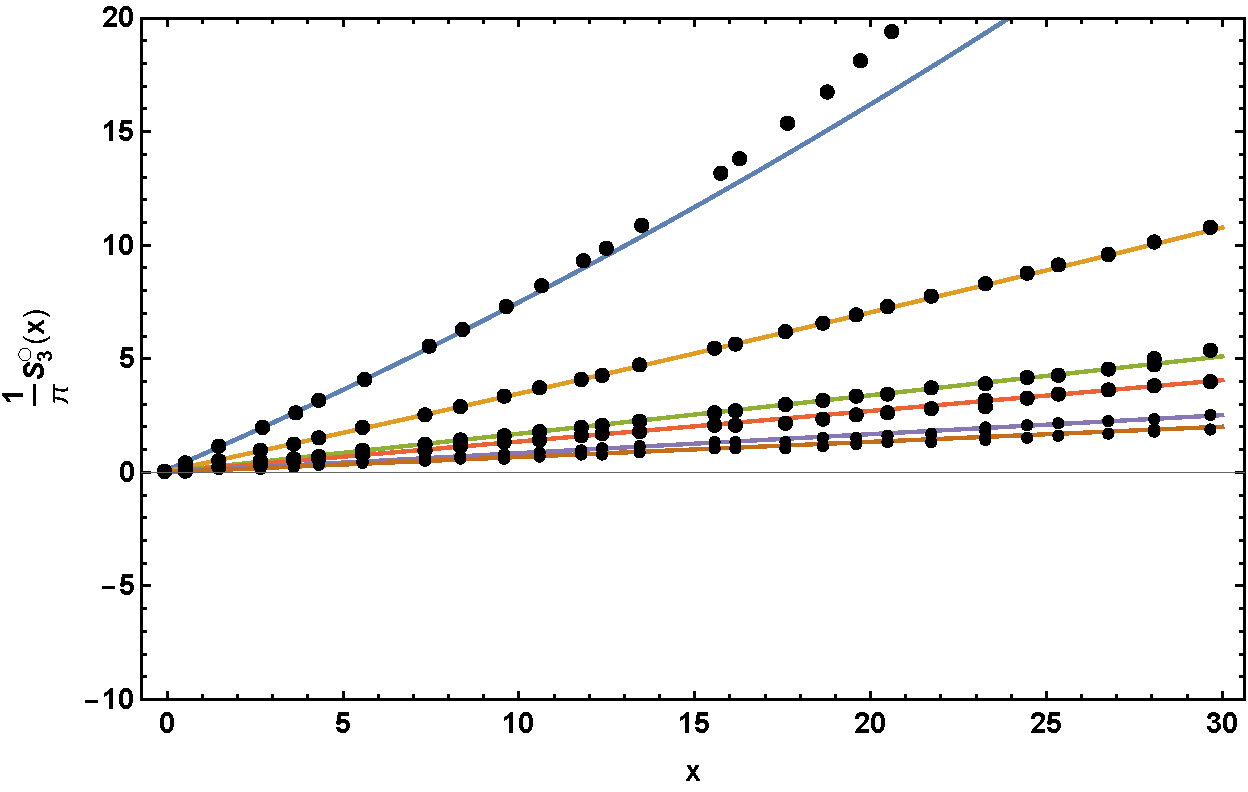
\includegraphics[width=.8\textwidth]{figs/S3_figure.pdf}
\caption{Plot of spherical L\"uscher as a function of $x$ for $N=10,20,40,50,80,100$.  Black points are actual numerical calcualtions (see text).\label{fig:S3 figure}}
\end{figure}
I also provide numerical calculations (black dots) that were determined in the following manner:
\begin{itemize}
\item I set $|a_0|\to\infty$
\item Given some $N$, I solve for the zeros of eq.~\eqref{eqn:finally there}.  This provides me with a list of $x$ values corresponding to the eigenvalues of the Schr\"odinger equation
\item I feed these values through a numerical implementation of the spherical L\"uscher formula, obtaining the black points shown in \autoref{fig:S3 figure}
\end{itemize}
The level of agreement between the black points and the curves suggest that I'm doing something right.  We can now improve on the spherical L\"uscher result by subtracting off this dependence.

\section{Finite range interaction}
In the previous section a contact interaction was used as the potential and the ensuing corrections to the spherical L\"uscher formula were derived with such an interaction.  Here we consider if such corrections can be applied in general, i.e. to finite-range potentials.

\subsection{Separable Gaussians}

We assume a \emph{God-given} potential of the form
\begin{align}
\langle \bm p'|\hat V|\bm b\rangle &=V(p',p)= \frac{2\pi C_0}{\mu}f(p')f(p)\label{eqn:god potential}\\
f(p)&=\exp\left(-\frac{\pi (pr)^2}{32}\right)\nonumber\\
C_0^{-1}&=\frac{1}{a_0}-\frac{4}{\pi  r}\nonumber\ ,
\end{align}
where $a_0$ and $r$ are parameters of the potential.
The phase shift for this potential can be analytically determined (see \autoref{sect:phase shift}), 
\begin{equation}
p\cot\delta(p)=\frac{1}{f(p)^2}\left(-\frac{1}{a_0}+\frac{2 p}{\sqrt{\pi}} F\left(\frac{1}{4} p \sqrt{\pi } r\right)\right)\ ,
\end{equation}
where $F(x)$ is Dawson's integral.  The corresponding effective range expansion (see \autoref{sect:ERE}),
\begin{equation}
p\cot\delta(p)=-\frac{1}{a_0}+\frac{p^2 r}{2}-\frac{1}{48} \pi  p^4 r^3+\ldots\ ,
\end{equation}
shows that the parameters $a_0$ and $r$ correspond to the scattering length and effective range, respectively.  Finally, the (dimensionless) eigenstates $x$ of the Schr\"odinger equation with this potential in a discretized box satisfy the self-consistency equation (\autoref{sect:eigenvalues})
\begin{equation}\label{eqn:SE}
-\frac{L}{a_0}+\frac{4L}{\pi  r}=\frac{1}{\pi}\sum_{\bm n\in\mathrm{B.Z.}}\frac{f\left(\bm n\right)^2}{\bm n^2-x}\ ,
\end{equation}
where
\begin{equation}
f(\bm n)=\exp\left(-\frac{\pi ^3  r^2}{8 L^2}\bm n^2\right)\ .
\end{equation}

\subsubsection{$^1S_0$ channel}
Here I use the following parameters,
\begin{align*}
a_0&=-18.1\ \mathrm{ fm}\\
r&=2.8\ \mathrm{ fm}\\
L&=50\ \mathrm{ fm}\ .
\end{align*}
We perform calculations with $N=16$ and $N=32$, where in each case we calculate the values of $x$ that satisfy eq.~\eqref{eqn:SE} and feed the resulting results through both dispersion L\"uscher,
\begin{equation}\label{eqn:dispersion luscher}
\frac{1}{\pi L}S^{\square N}_3(x)=\frac{1}{\pi L}\left(\sum_{\bm n\in\mathrm{B.Z.}}\frac{1}{\bm n^{2}-x}-\mathcal{L}^\square_3\frac{N}{2}\right)\ ,
\end{equation}
and spherical L\"uscher,
\begin{equation}
\frac{1}{\pi L}S^\bigcirc_3(x)=\lim_{\eta \to\infty}\frac{1}{\pi L}\left(\sum_{\bm n}^{|\bm n|<\eta / 2} \frac{1}{\bm n^{2}-x}-\mathcal{L}^\bigcirc_3\frac{\eta}{2}\right)\ .
\end{equation}
\autoref{fig:1s0 gaussian}
\begin{figure}
\includegraphics[width=.5\textwidth]{figs/pcotd_1S0_gaussian.pdf}\includegraphics[width=.5\textwidth]{figs/delta_1S0_gaussian.pdf}
\caption{``$^1S_0$" case.  Dashed line is exact.  Shown is spherical L\"uscher for $N=16$ (light blue) and $N=32$ (dark blue), and corresponding dispersion L\"uscher for $N=16$ (light red) and $N=32$ (dark red). In all cases, spherical L\"uscher is closer to the exact solution (the $N=32$ (dark blue) results are essentially on the exact line).  The corrections from the previous section would move light (dark) blue to light (dark) red, which would make spherical L\"uscher worse!\label{fig:1s0 gaussian}}
\end{figure}
shows these numerical results.  PLEASE READ THE CAPTION CAREFULLY!  What \autoref{fig:1s0 gaussian} shows is that spherical L\"uscher is the better approximation, and that the corrections derived in the previous section (which would move spherical L\"uscher to dispersion L\"uscher) would make the result \emph{worse}!

\subsubsection{$^3S_1$ channel}
Here I use the following parameters,
\begin{align*}
a_0&=5.4\ \mathrm{ fm}\\
r&=1.8\ \mathrm{ fm}\\
L&=50\ \mathrm{ fm}\ .
\end{align*}
The system now has a bound state and so Nyquist's theorem says that $\delta(0)=\pi$.
\begin{figure}
\includegraphics[width=.5\textwidth]{figs/pcotd_3S1_gaussian.pdf}\includegraphics[width=.5\textwidth]{figs/delta_3S1_gaussian.pdf}
\caption{``$^3S_1$" case.  Dashed line is exact.  Shown is spherical L\"uscher for $N=16$ (light blue) and $N=32$ (dark blue), and corresponding dispersion L\"uscher for $N=16$ (light red) and $N=32$ (dark red). As in the $^1S_0$ case (\autoref{fig:1s0 gaussian}), spherical L\"uscher is closer to the exact solution. \label{fig:3s1 gaussian} }
\end{figure}
We find the same behavior as in the $^1S_0$ case; namely, spherical L\"uscher is the better approximation to the exact result!

\subsection{Christopher's separable potential}
I also repeat the analysis using Christopher's potential which has a slower falloff in $p^2$ and one can also easily tune a bound state into the expression.  He defines it as
\begin{equation}\label{eqn:koerber potential}
V\left(\boldsymbol{p}^{\prime}, \boldsymbol{p}\right)=-g^{*}\left(\boldsymbol{p}^{\prime}\right) g(\boldsymbol{p}), \quad \quad \quad g(\boldsymbol{p})=\overline{g} \sqrt{8 \pi} \frac{M^{3}}{\left(\boldsymbol{p}^{2}+M^{2}\right)^{2}}, \quad M, \overline{g} \in \mathbb{R}\ ,
\end{equation}
where
\begin{equation}
\overline{g}=\frac{2 M(\gamma+M)^{2}}{\sqrt{\mu M^{3}\left(\gamma^{2}+5 M^{2}+4 \gamma M\right)}}\ .
\end{equation}
If one has a target binding energy $B$ (e.g. $B=2.2$ MeV), then one defines $\gamma=\sqrt{2\mu B}$.  Christopher has derived the phase-shift relation for this potential, and I trust his results, so I just state the result here,
\begin{multline}
p\cot\delta(p) = -\frac{5|\overline{g}|^{2} \mu M-4 M^{2}}{16|\overline{g}|^{2} \mu}+\frac{15|\overline{g}|^{2} \mu+16 M}{16|\overline{g}|^{2} \mu M} p^{2}+\frac{5|\overline{g}|^{2} \mu+24 M}{16|\overline{g}|^{2} \mu M^{3}} p^{4}\\
+\frac{|\overline{g}|^{2} \mu+16 M}{16|\overline{g}|^{2} \mu M^{5}} p^{6}+\frac{ p^{8}}{4|\overline{g}|^{2} \mu M^{6}}\ .
\end{multline}
As opposed to the separable Gaussian potential from the previous section which has an infinite number of shape parameters, Christopher's potential has only a finite number of shape parameters (up to $p^8$).  A little investigation easily shows that the (dimensionless) eigenvalues $x$ of the Schr\"odinger equation with this interaction satisfies this self-consistency equation,
\begin{equation}
1-\frac{1}{\pi L}\sum_{\bm n\in\mathrm{B.Z.}}\frac{\frac{\mu}{2\pi}\left|g\left(\frac{2\pi}{L}\bm n\right)\right|^2}{\bm n^2-x}=0\ .
\end{equation}
I use the following parameters in this calculation,
\begin{align*}
M&=13.6\ \mathrm{ fm}^{-1}\\
\gamma&=.23\ \mathrm{ fm}^{-1}\\
\mu&=2.371678\ \mathrm{ fm}^{-1}\\
L&=10\ \mathrm{ fm}\ .
\end{align*}
and in this case, I have to do calculations with $N=32$ and $N=64$ to get something comparable to the Gaussian results. \autoref{fig:3s1 koerber} shows our results.
\begin{figure}
\includegraphics[width=.5\textwidth]{figs/pcotd_3S1_koerber.pdf}\includegraphics[width=.5\textwidth]{figs/delta_3S1_koerber.pdf}
\caption{Results using Christopher's potential in eq.~\eqref{eqn:koerber potential}.  Dashed line is exact.  Shown is spherical L\"uscher for $N=32$ (light blue) and $N=64$ (dark blue), and corresponding dispersion L\"uscher for $N=32$ (light red) and $N=64$ (dark red). Again, spherical L\"uscher is closer to the exact solution. \label{fig:3s1 koerber} }
\end{figure}
We reach the same conclusion as in the Gaussian case:  spherical L\"uscher is the better approximation.  

\subsection{Corrections to spherical L\"uscher in the case of finite-range interactions}
As we'll find out, corrections to spherical L\"uscher in the case of finite-range interactions will depend on the details of the interaction, which is unfortunate.  To keep the presentation simple, we'll again assume a separable interaction of the form
\begin{equation}
V(\bm p',\bm p)=\frac{2\pi}{\mu} \mathcal{C} f(\bm p')f(\bm p)\ .
\end{equation}
We label the discrete box eigenvalues as $x_N$.  They satisfy
\begin{equation}\label{eqn:x_N}
1+\frac{\mathcal{C}}{\pi L}\sum_{\bm n\in\mathrm{B.Z.}}\frac{f\left(\frac{2\pi}{L}\bm n\right)^2}{\bm n^2-x_N}=0\ .
\end{equation}
Recall that $\bm n\in\mathrm{B.Z.}$ represents $\bm n\in\ (-N/2,N/2]^3$.  Let us now take the continuum limit (while holding $L$ fixed).  This is equivalent to $N\to \infty$.  We label the (continuum) box eigenvalues in this case as $x_\infty$.  They satisfy
\begin{equation}\label{eqn:x_infinity}
1+\frac{\mathcal{C}}{\pi L}\sum_{\bm n\in(-\infty,\infty]^3}\frac{f\left(\frac{2\pi}{L}\bm n\right)^2}{\bm n^2-x_\infty}=0\ .
\end{equation}
Up to finite-volume corrections, these are the energies that, when be pushed through spherical L\"uscher, provide information on the infinite-volume, continuum phase shifts\footnote{From now on, I make no distinction between \emph{cartesian} and \emph{spherical} L\"uscher.  They are the same thing, i.e. $S^\square_3(x)=S^\bigcirc_3(x)=S_3(x)$.}
\begin{equation}
p\cot\delta=\frac{1}{\pi L}S_3(x_\infty)\ .
\end{equation}
We now add the spherical L\"uscher equation to both sides of eq.~\eqref{eqn:x_infinity} (and multiply both sides by $L$),
\begin{equation}\label{eqn:x_infinity 2}
L+\lim_{N\to\infty}\frac{1}{\pi}\left[\sum_{\bm n\in(-N/2,N/2]^3}\frac{\mathcal{C}f\left(\frac{2\pi}{L}\bm n\right)^2+1}{\bm n^2-x_\infty}-\mathcal{L}^\square_3\frac{N}{2}\right]=\frac{1}{\pi}S_3(x_\infty)\ .
\end{equation}
Now we set $x_\infty=x_N+\delta x$ in the LHS and assume that $|\delta x/x_N|\ll 1$.  We expand the LHS in $\delta x$,
\begin{multline}
L+\lim_{N\to\infty}\frac{1}{\pi}\left[\sum_{\bm n\in(-N/2,N/2]^3}\frac{\mathcal{C}f\left(\frac{2\pi}{L}\bm n\right)^2+1}{\bm n^2-x_N}-\mathcal{L}^\square_3\frac{N}{2}\right]\\
+ \frac{\delta x}{\pi}\sum_{\bm n\in(-\infty,\infty]^3}\frac{\mathcal{C}f\left(\frac{2\pi}{L}\bm n\right)^2+1}{\left(\bm n^2-x_N\right)^2}+\mathcal{O}(\delta x^2)\\
=L+\frac{1}{\pi}\sum_{\bm n\in(-\infty,\infty]^3}\frac{\mathcal{C}f\left(\frac{2\pi}{L}\bm n\right)^2}{\bm n^2-x_N}+\frac{1}{\pi}S_3(x_N)\\
+ \frac{\delta x}{\pi}\sum_{\bm n\in(-\infty,\infty]^3}\frac{\mathcal{C}f\left(\frac{2\pi}{L}\bm n\right)^2+1}{\left(\bm n^2-x_N\right)^2}+\mathcal{O}(\delta x^2)=\frac{1}{\pi}S_3(x_\infty)\ .
\end{multline}
We now split the first sum into $\sum_{\bm n\in(-\infty,\infty]^3}=\sum_{\bm n\in\mathrm{B.Z.}}+\sum_{\bm n\notin\mathrm{B.Z.}}$ and use eq.~\eqref{eqn:x_N} to get
\begin{multline}
S_3(x_\infty)=S_3(x_N)+\sum_{\bm n\notin\mathrm{B.Z.}}\frac{\mathcal{C}f\left(\frac{2\pi}{L}\bm n\right)^2}{\bm n^2-x_N}
+ \delta x\sum_{\bm n\in(-\infty,\infty]^3}\frac{\mathcal{C}f\left(\frac{2\pi}{L}\bm n\right)^2+1}{\left(\bm n^2-x_N\right)^2}\\+\mathcal{O}(\delta x^2)\ .
\end{multline}
Using the $\mathcal{I}_\alpha(x)$ coefficients defined earlier, we have
\begin{multline}
S_3(x_\infty)=S_3(x_N)+\sum_{\bm n\notin\mathrm{B.Z.}}\frac{\mathcal{C}f\left(\frac{2\pi}{L}\bm n\right)^2}{\bm n^2-x_N}
+ \delta x\left(\mathcal{I}_2(x_n)+\sum_{\bm n\in(-\infty,\infty]^3}\frac{\mathcal{C}f\left(\frac{2\pi}{L}\bm n\right)^2}{\left(\bm n^2-x_N\right)^2}\right)\\+\mathcal{O}(\delta x^2)\ .
\end{multline}
The $\delta x$-\emph{independent} correction (second term on the RHS above) is dependent on the details of the interaction.  Introducing dimensionful quantities, this correction is
\begin{equation}
\frac{1}{\pi L}\sum_{\bm n\notin\mathrm{B.Z.}}\frac{\mathcal{C}f\left(\frac{2\pi}{L}\bm n\right)^2}{\bm n^2-x_N}
=-\frac{1}{L^3}\sum_{\bm p_n\notin\mathrm{B.Z.}}\frac{V(\bm p_n,\bm p_n)}{E_N-\frac{\bm p_n^2}{2\mu}}\ ,
\end{equation}
where $\bm p_n=\frac{2\pi \bm n}{L}$ and $E_N=\frac{2\pi^2 x_N}{\mu L^2}$. 
Even though this expression was derived using a separable interaction, I believe it actually holds for general potentials and suggests that the correction is a tadpole diagram. 


\appendix
\section{Phase shift, ERE, and eigenvalues of potential given in eq.~\eqref{eqn:god potential}\label{sect:god potential}}
We first solve for the T-matrix,
\begin{displaymath}
T = V+VG_0 T\ .
\end{displaymath}
Because the potential in eq.~\eqref{eqn:god potential} is separable, the T-matrix can be easily solved,
\begin{align}
\langle \bm p'|T|\bm p\rangle &= \frac{V(p',p)}{1-I(E)}\label{eqn:T-matrix solution}\\
I(E)&=\frac{m}{2\pi^2}\int dq\frac{q^2V(q,q)}{mE-q^2+i\epsilon}\ .
\end{align}
The integral can be simplified further,
\begin{multline}
I(E)=-\frac{m}{2\pi^2}\int dq\ V(q,q)+\frac{m(mE)}{2\pi^2}\int dq\frac{V(q,q)}{mE-q^2+i\epsilon}\\
=-\frac{2C_0}{\pi}\int dq\  f(q)^2\\
+\frac{2C_0 mE}{\pi}\int dq\ f(q)^2\left(\frac{\mathcal{P}}{mE-q^2}-i\pi \delta(mE-q^2)\right)
\ .
\end{multline}

\subsection{Phase shift\label{sect:phase shift}}
The full on-shell T-matrix is when $\bm p'=\bm p=\sqrt{mE}$ and is defined as
\begin{equation}
T(p^2=mE)=\frac{-4\pi/m}{p\cot \delta(p)-ip}\ .
\end{equation}
Equating this to eq.~\eqref{eqn:T-matrix solution} and manipulating some terms gives
\begin{equation}
\frac{-4\pi/m}{p\cot \delta(p)-ip}=
\frac{4\pi/m}{\frac{1}{f(p)^2}\left(\frac{1}{C_0}+\frac{2}{\pi}\int dq\  f(q)^2-\frac{2p^2}{\pi}\int dq\ f(q)^2\frac{\mathcal{P}}{p^2-q^2}\right)+ip}\ .
\end{equation}
This means that
\begin{equation}
p\cot\delta(p)=\frac{1}{f(p)^2}\left(\frac{-1}{C_0}-\frac{2}{\pi}\int dq\  f(q)^2+\frac{2p^2}{\pi}\int dq\ f(q)^2\frac{\mathcal{P}}{p^2-q^2}\right)\ .
\end{equation}
We now use the explicit form of $f(p)$ given in eq.~\eqref{eqn:god potential} and perform the integrals,
\begin{equation}
\boxed{
p\cot\delta(p)=\frac{1}{f(p)^2}\left(-\frac{1}{a_0}+\frac{2 p F\left(\frac{1}{4} p \sqrt{\pi } r\right)}{\sqrt{\pi
   }}\right)}\ .
\end{equation}
Here $F(x)$ is the Dawson integral.

\subsection{ERE\label{sect:ERE}}
We now perform a series expansion in $p$, which gives the effective range expansion,
\begin{equation}
p\cot\delta(p)=-\frac{1}{a_0}+\frac{p^2 r}{2}-\frac{1}{48} \pi  p^4 r^3+\ldots
\end{equation}
Thus we see that the parameters $a_0$ and $r$ correspond to the scattering length and effective range, respectively.

\subsection{Solution to Schr\"odinger's equation in a disretized box\label{sect:eigenvalues}}
We start with the integral form of the Schr\"odinger's equation,
\begin{multline}
\langle \bm p|\psi\rangle = \frac{1}{E-p^2/m}\langle \bm p|\hat V|\psi\rangle= 
\frac{1}{L^3}\frac{1}{E-p^2/m} \sum_{\bm q\in\mathrm{B.Z.}}\langle\bm p|\hat V|\bm q\rangle\langle\bm q|\psi\rangle\\
=\frac{1}{L^3}\frac{4\pi}{m}\frac{C_0 f(p)}{E-p^2/m} \left[\sum_{\bm q\in\mathrm{B.Z.}}f(q)\langle\bm q|\psi\rangle\right]
\ .
\end{multline}
Now multiply by $f(p)$ from the left and sum over $\bm p$,
\begin{equation}
\sum_{\bm p\in\mathrm{B.Z.}} f(p)\langle\bm p|\psi\rangle=\left\{\frac{1}{L^3}\sum_{\bm p\in\mathrm{B.Z.}}\frac{4\pi}{m}\frac{C_0 f(p)^2}{E-p^2/m} \right\} \left[\sum_{\bm q\in\mathrm{B.Z.}}f(q)\langle\bm q|\psi\rangle\right]\ .
\end{equation}
Using the same manipulations as was done in \autoref{sect:disguise} one finds that the eigenvalues $E$ must satisfy
\begin{equation}
1-\frac{1}{L^3}\frac{4\pi}{m}\sum_{\bm p\in\mathrm{B.Z.}}\frac{C_0 f(p)^2}{E-p^2/m}=0\ .
\end{equation}
Replacing $\bm p \to \frac{2\pi}{L}\bm n$ and $x=\frac{mEL^2}{4\pi^2}$, and a little more manipulation, one finds
\begin{equation}
-\frac{L}{C_0}=\boxed{-\frac{L}{a_0}+\frac{4L}{\pi  r}=\frac{1}{\pi}\sum_{\bm n\in\mathrm{B.Z.}}\frac{f\left(\bm n\right)^2}{\bm n^2-x}}\ ,
\end{equation}
where
\begin{equation}
f(\bm n)=\exp\left(-\frac{\pi ^3  r^2}{8 L^2}\bm n^2\right)\ .
\end{equation}

%\clearpage
%\bibliography{references}

\end{document}  
